% =====================================================================
% Three-panel composite figure: A + B + C (black-and-white, English)
% Compile with: xelatex figure_combined.tex
% =====================================================================
\documentclass[10pt,a4paper]{article}
\usepackage[a4paper,margin=1.5cm,top=1.2cm,bottom=1.2cm]{geometry}
\usepackage{fontspec}
\usepackage{tikz}
\usepackage{booktabs}
\usepackage{array}
\usepackage{graphicx}
\usepackage{amsmath}
\usepackage{xcolor}

\usetikzlibrary{arrows.meta,positioning,calc,bending,spath3}

% --- Fonts ---
\setmainfont{Arial}
\setsansfont{Arial}

% --- Gray tones for B/W ---
\definecolor{boxgray}{HTML}{F5F5F5}
\definecolor{bordergray}{HTML}{888888}

\pagestyle{empty}
\setlength{\parindent}{0pt}

\begin{document}

% ============================================================
% A. Path diagram with statistical results
% ============================================================
\noindent
{\large\textbf{A.}}\\[2pt]

\begin{center}
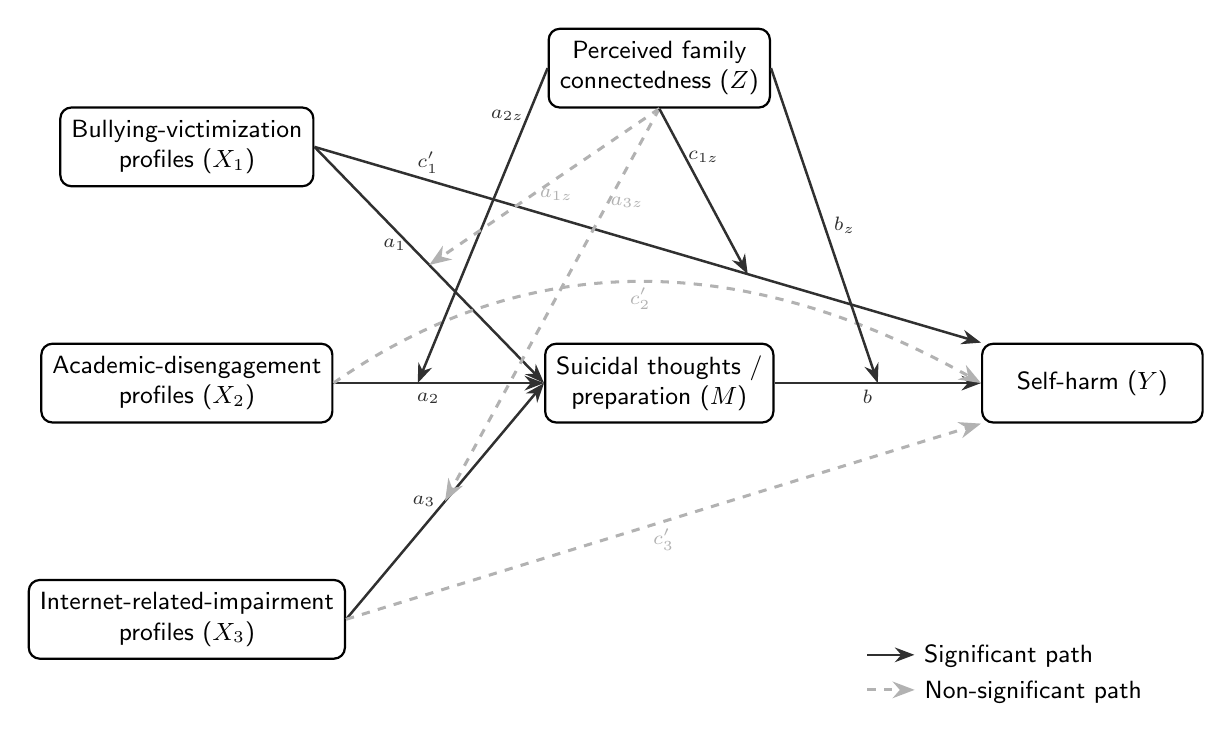
\begin{tikzpicture}[
    node distance=1.2cm and 2.8cm,
    box/.style={
        rectangle, rounded corners=4pt, draw=black, line width=0.8pt,
        fill=white, minimum width=2.8cm, minimum height=1.0cm,
        align=center, font=\small\sffamily, inner sep=4pt
    },
    % Significant path: solid dark gray
    sigline/.style={
        ->, >=Stealth, line width=0.9pt, darkgray!75!black
    },
    % Non-significant path: dashed gray
    nsline/.style={
        ->, >=Stealth, line width=1.1pt, gray!60, dashed
    },
    lbl/.style={
        font=\scriptsize\sffamily, align=center, fill=none, inner sep=1pt
    }
]

% === Nodes ===
\node[box] (BV)  at (-4, 3)  {Bullying-victimization\\profiles ($X_1$)};
\node[box] (AD)  at (-4, 0)  {Academic-disengagement\\profiles ($X_2$)};
\node[box] (IRI) at (-4, -3) {Internet-related-impairment\\profiles ($X_3$)};

\node[box] (M)   at (2, 0)   {Suicidal thoughts /\\preparation ($M$)};
\node[box] (Y)   at (7.5, 0) {Self-harm ($Y$)};

\node[box] (Z)   at (2, 4.0) {Perceived family\\connectedness ($Z$)};

% ============================================================
% === a paths: X -> M
% ============================================================
% BV -> M: a_1
\draw[sigline] (BV.east) -- (M.west)
    node[lbl, pos=0.35, below=2pt] {$a_1$};

% AD -> M: a_2
\draw[sigline] (AD.east) -- (M.west)
    node[lbl, pos=0.45, below=2pt] {$a_2$};

% IRI -> M: a_3
\draw[sigline] (IRI.east) -- (M.west)
    node[lbl, pos=0.5, left=2pt] {$a_3$};

% ============================================================
% === b path: M -> Y
% ============================================================
\draw[sigline] (M.east) -- (Y.west)
    node[lbl, pos=0.45, below=1pt] {$b$};

% ============================================================
% === Direct effects: X -> Y (c' paths)
% ============================================================
% AD -> Y: c'_2 (non-significant, arc)
\draw[nsline] (AD.east) to[out=35,in=-210] coordinate[pos=0.52] (AD_Y_arc_mid) (Y.west)
    node[lbl, pos=0.5, above=25pt, xshift=50pt] {$c'_2$};

% BV -> Y: c'_1
\draw[sigline] (BV.east) -- (Y.north west)
    node[lbl, pos=0.17, above=1pt] {$c'_1$};

% IRI -> Y: c'_3
\draw[nsline] (IRI.east) -- (Y.south west)
    node[lbl, pos=0.50, below=1pt] {$c'_3$};

% ============================================================
% === Stage 1 Moderation: Z moderates a paths (X->M)
% ============================================================
% Z -> AD->M: a_2z (significant)
\coordinate (AD_M_mid) at ($(AD.east)!0.4!(M.west)$);
\draw[sigline] (Z.west) -- (AD_M_mid)
    node[lbl, pos=0.15, left=0.1pt] {$a_{2z}$};

% Z -> BV->M: a_1z (non-significant)
\coordinate (BV_M_mid) at ($(BV.east)!0.5!(M.west)$);
\draw[nsline] (Z.south) -- (BV_M_mid)
    node[lbl, pos=0.55, right=1pt] {$a_{1z}$};

% Z -> IRI->M: a_3z (marginally ns)
\coordinate (IRI_M_mid) at ($(IRI.east)!0.5!(M.west)$);
\draw[nsline] (Z.south) -- (IRI_M_mid)
    node[lbl, pos=0.15, below=9pt] {$a_{3z}$};

% ============================================================
% === Stage 2 Moderation: Z moderates b path (M->Y)
% ============================================================
\coordinate (M_Y_mid) at ($(M.east)!0.5!(Y.west)$);
\draw[sigline] (Z.east) -- (M_Y_mid)
    node[lbl, pos=0.5, right=2pt] {$b_z$};

% ============================================================
% === c' path Moderation: Z moderates direct effects (X->Y)
% ============================================================
% Z -> BV->Y: c_{1z} (significant)
\coordinate (BV_Y_mid) at ($(BV.east)!0.65!(Y.north west)$);
\draw[sigline] (Z.south) -- (BV_Y_mid)
    node[lbl, pos=0.5, above=9pt] {$c_{1z}$};

% Z -> IRI->Y: c_{3z} (non-significant)
%\coordinate (IRI_Y_mid) at ($(IRI.east)!0.65!(Y.south west)$);
%\draw[nsline] (Z.south) -- (IRI_Y_mid) node[lbl, pos=0.30, left=0.1pt] {$c_{3z}$};

% ============================================================
% === Legend ===
% ============================================================
\node[font=\small\sffamily, align=left, anchor=north west] at (4.5, -3.2) {
    \tikz\draw[sigline] (0,0) -- (0.6,0); Significant path\\[2pt]
    \tikz\draw[nsline] (0,0) -- (0.6,0); Non-significant path
};

\end{tikzpicture}
\end{center}

\vspace{0.2em}

% ============================================================
% B + C side by side
% ============================================================
\noindent
\begin{minipage}[t]{0.50\textwidth}
{\large\textbf{B.}}\\[3pt]
\renewcommand{\arraystretch}{1.05}
{\scriptsize
\begin{tabular}{@{}p{0.7cm}p{1.6cm}p{2.5cm}p{1.4cm}p{1.2cm}@{}}
\toprule
\textbf{Symbol} & \textbf{Path} & \textbf{Test / Est.\ (BC 95\% CI)} & \textbf{$p$ Value} & \textbf{Direction} \\
\midrule
\multicolumn{4}{@{}l}{\textit{$a$-path}} \\[1pt]
$a_1$ & $X_1 \to M$ & $\chi^2(3)=24.73$ & $<.001^{***}$ & Positive \\
$a_2$ & $X_2 \to M$ & $\chi^2(3)=17.10$ & $<.001^{***}$ & Positive\\
$a_3$ & $X_3 \to M$ & $\chi^2(3)=14.40$ & $.002^{**}$ & Positive\\
\midrule
\multicolumn{4}{@{}l}{\textit{$b$-path}} \\[1pt]
$b$   & $M \to Y$   & $.460[.39,.54]$   & $<.001^{***}$ & Positive\\
\midrule
\multicolumn{4}{@{}l}{\textit{Direct effects (bypassing $M$)}} \\[1pt]
$c'_1$ & $X_1 \to Y$ & $\chi^2(3)=46.11$ & $<.001^{***}$ & Positive \\
$c'_2$ & $X_2 \to Y$ & $\chi^2(3)=0.29$  & $.963$ & n.s. \\
$c'_3$ & $X_3 \to Y$ & $\chi^2(3)=6.30$  & $.098$ & n.s. \\
\midrule
\multicolumn{4}{@{}l}{\textit{Moderation effects}} \\[1pt]
$a_{1z}$ & $Z \times a_1$ & $\chi^2(3)=2.68$  & $.444$  & n.s.\\
$a_{2z}$ & $Z \times a_2$ & $\chi^2(3)=8.14$  & $.043^{*}$ & Negative\\
$a_{3z}$ & $Z \times a_3$ & $\chi^2(3)=7.31$  & $.063$ & n.s. \\
$b_z$    & $Z \times b$   & $-.074$ [$-.12$, $-.02$] & $.003^{**}$ & Negative\\
$c_{1z}$ & $Z \times c'_1$ & $\chi^2(3)=14.12$ & $.003^{**}$ & Positive  \\
\bottomrule
\end{tabular}}
\end{minipage}
\hfill
\begin{minipage}[t]{0.47\textwidth}
{\large\textbf{C.}}\\[7pt]

\includegraphics[width=\linewidth]{figure_C_conditional_indirect.pdf}
\end{minipage}

\end{document}
